\documentclass[a4paper,12pt]{article} 
\usepackage[T2A]{fontenc}			
\usepackage[utf8]{inputenc}			
\usepackage[english,russian]{babel}	
\usepackage{amsmath,amsfonts,amssymb,amsthm,mathrsfs,mathtools} 
\usepackage{cancel}
\usepackage{multirow}
\usepackage[colorlinks, linkcolor = blue]{hyperref}
\usepackage{upgreek}\usepackage[left=2cm,right=2cm,top=2cm,bottom=3cm,bindingoffset=0cm]{geometry}
\usepackage{graphicx,wrapfig,subfig}
\usepackage{tikz}
\usepackage{pgfplots}
\usepackage{xcolor}
\author{Дорогинин Д.В.\\
Группа Б02-825}
\title{3.5.1. Изучение плазмы газового разряда в неоне.}
\date{}
\begin{document}

\begin{titlepage}
	\centering
	\vspace{5cm}
	{\scshape\LARGE Московский физико-технический институт \par}
	\vspace{4cm}
	{\scshape\Large Лабораторная работа 3.5.1 \par}
	\vspace{1cm}
	{\huge\bfseries Изучение плазмы газового разряда в неоне. \par}
	\vspace{1cm}
	\vfill
\begin{flushright}
	{\large выполнил студент 924 группы ФОПФ}\par
	\vspace{0.3cm}
	{\LARGE Панферов Андрей}
\end{flushright}
	

	\vfill

% Bottom of the page
	Долгопрудный, 2020 г.
\end{titlepage}

\textbf{Цель работы}: изучение вольт-амперной характеристики тлеющего разряда, изучение свойств плазмы методом зондовых характеристик.


\textbf{В работе используются}: стеклянная газоразрядная трубка, наполненная изотопом неона, высоковольтный источник питания (ВИП), источник питания постоянного тока, делитель напряжения, резистор, потенциометр, амперметры, вольтметры, переключатели.
\section*{Теория}
\subsection*{Плазма}
В ионизированном газе поле ионов <<экранируется>> электронами. Для поля $\mathbf{E}$ и плотности $\rho$ электрического заряда
$$
\text{div}~\mathbf{E} = 4 \pi \rho,
$$
а с учётом сферической симметрии и $\mathbf{E} = -\text{grad}~\varphi$:
\begin{equation}
\dfrac{d^2 \varphi}{dr^2}+\dfrac{2}{r}\dfrac{d\varphi}{dr}=-4\pi \rho.
\end{equation}
Плотности заряда электронов и ионов (которые мы считаем бесконечно тяжёлыми и поэтому неподвижными)
\begin{equation}
\begin{array}{c}
\rho_e = -ne \cdot \exp\left(\dfrac{e\varphi}{kT_e}\right),\\
\rho_i = ne.
\end{array}
\end{equation}
Тогда из $(1)$ в предположении $\dfrac{e\varphi}{kT_e} \ll 1$ получим
\begin{equation}
\varphi = \dfrac{Ze}{r}e^{-r/r_D},
\end{equation}
где $r_D = \sqrt{\dfrac{kT_e}{4\pi n e^2}}$ -- \textit{радиус Дебая}. Среднее число ионов в сфере такого радиуса 
\begin{wrapfigure}{r}{4cm}
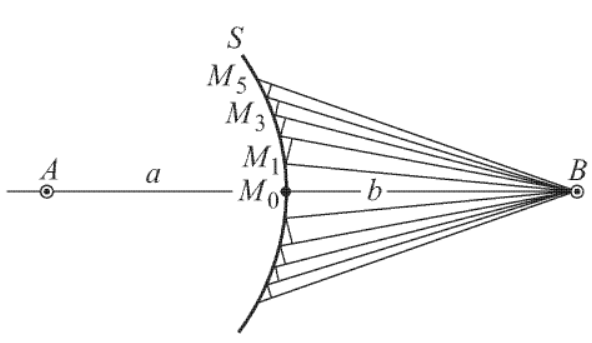
\includegraphics[scale=0.5]{2.png}
\end{wrapfigure}  
\begin{equation}
N_D = n\dfrac{4}{3}\pi r_D^2.
\end{equation}
Теперь выделим параллелепипед с плотностью $n$ электронов, сместим их на $x$. Возникнут поверхностные заряды $\sigma = nex$, поле от которых будет придавать электронам ускорение:
$$
\dfrac{d^2x}{dt^2}=-\dfrac{eE}{m}=-\dfrac{4\pi n e^2}{m}x.
$$ 
Отсюда получаем \textit{плазменную (ленгмюровскую) частоту} колебаний электронов:
\begin{equation}
\omega_p = \sqrt{\dfrac{4\pi ne^2}{m}}.
\end{equation}
\subsection*{Одиночный зонд}
При внесении в плазму уединённого проводника -- \textit{зонда} -- с потенциалом, изначально равным потенциалу точки плазмы, в которую его помещают, на него поступают токи электроннов и ионов:
\begin{equation}
\begin{array}{c}
I_{e0} = \dfrac{n \langle v_e \rangle}{4}eS,\\
I_{i0} = \dfrac{n \langle v_i \rangle}{4}eS,
\end{array}
\end{equation}
где $\langle v_e \rangle$ и $\langle v_i \rangle$ -- средние скорости электронов и ионов, $S$ -- площадь зонда, $n$ -- плотность электронов и ионов. Скорости электронов много больше скорости ионов, поэтому $I_{i0} \ll I_{e0}$. Зонд будет заряжаться до некоторого равновестного напряжения $-U_f$ -- \textit{плавающего потенциала}.\\
\begin{wrapfigure}{r}{5.5cm}
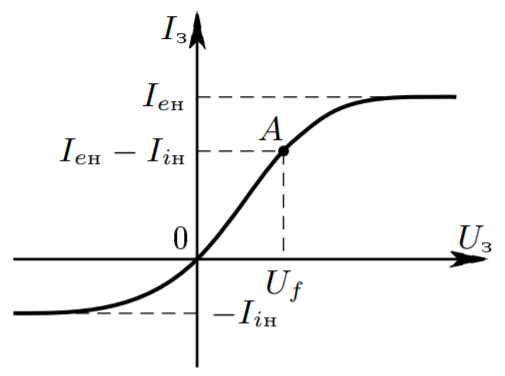
\includegraphics[scale=0.5]{3.png}
\end{wrapfigure}  
В равновесии ионный ток мало меняется, а электронный имеет вид
$$
I_e = I_0 \exp\left( -\dfrac{eU_f}{kT_e} \right).
$$
Будем подавать потенциал $U_\text{з}$ на зонд и снимать значение зондового тока $I_\text{з}$. Максимальное значение тока $I_{e\text{н}}$ -- электронный ток насыщения, а минимальное $I_{i\text{н}}$ -- ионный ток насыщения. Значение из эмпирической формулы Бомона:
\begin{equation}
I_{i\text{н}} = 0.4 neS \sqrt{\dfrac{2kT_e}{m_i}}.
\end{equation}
\subsection*{Двойной зонд}
Двойной зонд -- система из двух одинаковых зондов, расположенных на небольшом расстоянии друг от друга, между которыми создаётся разность потенциалов, меньшая $U_f$. Рассчитаем ток между ними вблизи $I=0$. При небольших разностях потенциалов ионные токи на оба зонда близки к току насыщения и компенсируют друг друга, а значит величина результирующего тока полностью связана с разностью электронных токов. Пусть потенциалы на зондах
$$
U_1 = -U_f + \Delta U_1,
$$
$$
U_2 = -U_f + \Delta U_2.
$$
Между зондами $U = U_2 - U_1 = \Delta U_2 - \Delta U_1$.
Через первый электрод
\begin{equation}
I_1 = I_{i\text{н}} + I_{e1} = I_{i\text{н}} - \dfrac{1}{4}neS\langle v_e\rangle \exp\left(-\dfrac{eU_f}{kT_e}\right)\exp\left(\dfrac{e\Delta U_1}{kT_e}\right)=I_{i\text{н}}\left(1 - \exp\left( \dfrac{e\Delta U_1}{kT_e} \right)\right).
\end{equation}
Аналогично через второй получим
\begin{equation}
I_2 = I_{i\text{н}}\left(1 - \exp\left( \dfrac{e\Delta U_2}{kT_e} \right)\right)
\end{equation}
  
Из $(7)$ и $(8)$ с учётом последовательного соединение зондов ($I_1 = -I_2 = I)$:
$$
\Delta U_1= \dfrac{kT_e}{e}\text{ln}\left(1 - \dfrac{I}{I_{i\text{н}}}\right)
$$
$$
\Delta U_2= \dfrac{kT_e}{e}\text{ln}\left(1 + \dfrac{I}{I_{i\text{н}}}\right)
$$

Тогда итоговые формулы для разности потенциалов и тока

\begin{equation}
U = \dfrac{kT_e}{e}\text{ln}\dfrac{1 - I/I_{i\text{н}}}{1 + I/I_{i\text{н}}}, 
I = I_{i\text{н}} \text{th}\dfrac{eU}{2kT_e}.
\end{equation}
Реальная зависимость выглядит несколько иначе и описывается формулой 
\begin{wrapfigure}{l}{7cm}
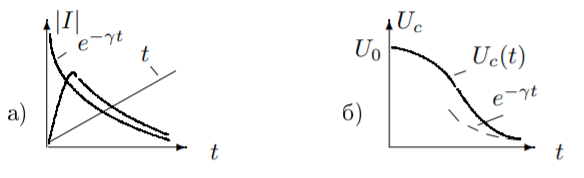
\includegraphics[scale=0.8]{4.png}
\vspace{+30pt}
\end{wrapfigure}
\begin{equation}
I = I_{i\text{н}} \text{th}\dfrac{eU}{2kT_e} + AU.
\end{equation}
Из этой формулы можно найти формулу для $T_e$: для $U=0$ мы найдём $I_{i\text{н}}$, продифференцируем в точке $U=0$ и с учётом $\text{th}~\alpha \approx \alpha$ при малых $\alpha$ и $A\rightarrow 0$ получим:
\begin{equation}
kT_e = \dfrac{1}{2}\dfrac{eI_{i\text{н}}}{\dfrac{dI}{dU}|_{U=0}}.
\end{equation}
\section*{Описание установки}
\begin{center}
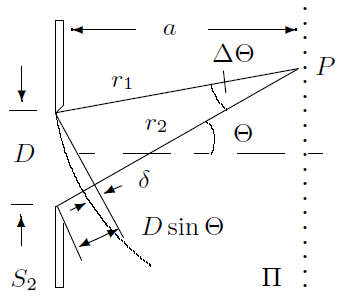
\includegraphics[scale=0.6]{1.png}
\end{center}
Стеклянная газоразрядная трубка имеет холодный (ненакаливаемый) полый катод, три анода и \textit{геттерный} узел -- стеклянный баллон, на внутреннюю повехность которого напылена газопоглощающая плёнка (\textit{геттер}). Трубка наполнена изотопом неона $^22$Ne при давлении 2 мм рт. ст. Катод и один из анодом (I и II) с помощью переключателя $\Pi_1$ подключается через балластный резистор $R_\text{б}$ ($\approx 450$ кОм) к регулируемому ВИП с выкодным напряжением до 5 кВ.\\
При подключении к ВИП анода-I между ним и катодом возникает газовый разряд. Ток разряда измеряется миллиамперметром $A_1$, а падение напряжения на разрядной трубке -- цифровым вольтметром $V_1$, подключённым к трубке черезе высокоомный (25 МОм) делитель напряжения с коэффициентом $(R_1+R_2)/R_2 = 10$.\\
При подключении к ВИП анода-II разряд возникает в пространстве между катодом и анодом-II, где находятся двойной зонд, используемый для диагностики плазмы положительного столба. Зонды изготовлены из молибденовой проволоки диаметром $d = 0.2$ мм и имеют длину $l = 5.2$ мм. Они подключены к источнику питания GPS через потенциометр $R$. Переключатель $\Pi_2$ позволяет изменять полярность напряжения на зондах. Величина напряжения на зондах изменяеься с помощью дискретного переключателя <<$V$>> выходного напряжения источника питания и потенциометра $R$, а измеряется цифровым вольтметром $V_2$. Для измерения зондового тока используется мультиметр $A_2$.
\section*{Ход работы}
Измеряем напряжение зажигания в лампе: $U_{\text{заж}} = 25.7\pm 0.2$ В.\\
С помощью вольтметра $V_1$ и амперметра $A_1$ снимаем ВАХ разряда $U_1=f(I_p)$ для тока в диапазоне $0.5 \div 5$ мА (см. Таблица 1).
Построим график:\\

\begin{center}
\begin{tikzpicture}[scale=1]
    	\begin{axis}[
    		axis lines = left,
        	xlabel = {$I$, mA},
        	ylabel = {$U$, V},
        	ylabel style={red, scale=1},
        	xlabel style={red, scale=1},
        	%xmin=0, xmax=9,
        	title={Зависимость $U(I)$},
        	legend style={at={(0.03,-0.4)},anchor=west},
        	table/col sep=semicolon,
    		]
    		\addplot +[blue, only marks]  plot[
			error bars/.cd,
			x dir = both,
			x fixed = 0.05,
			y dir = both,
			y fixed = 0.05,
		    ]
		    table[x=I, y=V]{Plasma.txt};
		    \addplot[color=red, domain=0.9:1.8]{-7.62 * (x - 1) + 35.36};
    	\end{axis}
    \end{tikzpicture}
\end{center}

По наклону определим максимальное сопротивление заряда (с учётом того, что вольтметр подключен через делитель напряжения с коэффициентом 10): $R_{max} = (7.6\pm 0.2)\cdot 10^4\text{Ом}$.\\
С помощью вольтмертра $V_2$ и амперметра $A_2$ снимем ВАХ двойного зонда $I_2 = f(U_2)$ при фиксированного токе разряда $I_p$ в трубке в диапозоне $-25 \div 25$ В, процессе измерений меняя полярность зонда при нулевом токе. Измерения проведём для $I_p = 5$ мА, $I_p = 3$ мА  и $I_p = 1.5$ мА (Таблица 2).\\
Результаты измерений представим на графиках с отцентрованными $\left(I_0 = \dfrac{1}{2}\sum I\right)$:
\newpage

\begin{minipage}{0.33\textwidth}
    \begin{center}
    \begin{tikzpicture}[scale=0.6]
        	\begin{axis}[
        		axis lines = middle,
            	xlabel = {$U, V$},
            	ylabel = {$I,\mu A$},
            	ylabel style={red, scale=1},
            	xlabel style={red, scale=1},
            	%xmin=0, xmax=9,
            	title={$I = 5mA$},
            	table/col sep=semicolon,
        		]
        		\addplot +[blue, only marks]  plot[
    			error bars/.cd,
    			x dir = both,
    			x fixed = 0.05,
    			y dir = both,
    			y fixed = 0.05,
    		    ]
    		    table[x=U1, y=I1]{Triple_probe_plot.txt};
    		    \addplot[color=red, domain=0:25]{0.775 * (x - 16) + 86.45 + 11.48};
        	\end{axis}
        \end{tikzpicture}
    \end{center}
\end{minipage}
\begin{minipage}{0.33\textwidth}
    \begin{center}
    \begin{tikzpicture}[scale=0.6]
        	\begin{axis}[
        		axis lines = middle,
            	xlabel = {$U, V$},
            	ylabel = {$I,\mu A$},
            	ylabel style={red, scale=1},
            	xlabel style={red, scale=1},
            	%xmin=0, xmax=9,
            	title={$I = 3mA$},
            	table/col sep=semicolon,
        		]
        		\addplot +[blue, only marks]  plot[
    			error bars/.cd,
    			x dir = both,
    			x fixed = 0.05,
    			y dir = both,
    			y fixed = 0.05,
    		    ]
    		    table[x=U2, y=I2]{Triple_probe_plot.txt};
    		    \addplot[color=red, domain=0:25]{0.592 * (x - 16) + 46.96 + 8.91};
        	\end{axis}
        \end{tikzpicture}
    \end{center}
\end{minipage}
\begin{minipage}{0.33\textwidth}
    \begin{center}
    \begin{tikzpicture}[scale=0.6]
        	\begin{axis}[
        		axis lines = middle,
            	xlabel = {$U, V$},
            	ylabel = {$I,\mu A$},
            	ylabel style={red, scale=1},
            	xlabel style={red, scale=1},
            	%xmin=0, xmax=9,
            	title={$I = 1.5mA$},
            	table/col sep=semicolon,
        		]
        		\addplot +[blue, only marks]  plot[
    			error bars/.cd,
    			x dir = both,
    			x fixed = 0.05,
    			y dir = both,
    			y fixed = 0.05,
    		    ]
    		    table[x=U3, y=I3]{Triple_probe_plot.txt};
    		    \addplot[color=red, domain=0:25]{0.288 * (x - 13) + 27.56};
        	\end{axis}
        \end{tikzpicture}
    \end{center}
\end{minipage}

$ $\\

Приближая кривые формулой $I = A \text{th}(BU) + CU$, найдём токи насыщения $I_{i\text{н}}$ и температуры электронов $T_e$.\\
Считая концентрации ионов и электронов равными, найдём их, пользуясь формулой (7). Рассчитаем плазменную частоты $\omega_p$ по формуле (5) и радиус Дебая $r_D$, оценим среднее число ионов в дебаевской сфера $N_D$ по формуле (4) и  степень ионизации $\alpha$, приняв $P\approx 1$ мбар, и занесём все результаты в таблицу.
\begin{table}[h!]
\centering
\begin{tabular}{|c|c|c|c|c|c|c|}
\hline
$I_p$, мА  & $T_e$, $10^3$ К   & $n_e$, $10^{14}$ м$^{-3}$ & $\omega_p$, $10^4$ рад/c & $r_D$, $10^{-4}$ м & $N_D, 10^5$ & $\alpha$, $10^{-7}$ \\ \hline
5.0   & $55\pm 6$ & $9.9\pm 8$                     & $1.87\pm 0.10$                   & $5.1\pm 0.3$                      & 5.5 & 75\\ \hline
3.0   & $47\pm 4$ & $5.8\pm 4$                     & $1.26\pm 0.08$                    & $6.2\pm 0.5$                      & 5.7 & 37\\ \hline
1.5   & $45\pm 4$ & $3.1\pm 2$                    & $1.04\pm 0.05$                     & $8.3 \pm 0.8$                     & 7.4 & 19\\ \hline
\end{tabular}
\end{table}

\section*{Вывод}

Полученные результаты по порядку совпадают с табличными (\href{https://en.wikipedia.org/wiki/Debye_length}{Wikipedia}). Все зависимости имеют именно такой вид, как предсказывала теория.
\newpage
\section*{Результаты измерений}
\begin{table}[h]
\centering
\begin{tabular}{|c|c|c|c|c|c|c|c|c|c|c|c|}
\hline
$U_1$, В & 27.72 & 27.68 & 28.26 & 28.56 & 29.8 & 31.55 & 35.36 & 35.3 \\ \hline
$I_p$, мА & 4.00 & 3.50  & 3.00  & 2.50 & 2.00  & 1.50  & 1.00  & 0.50 \\ \hline
\end{tabular}
\caption{Зависимость $U_1 = f(I_p)$.}
\end{table}

\begin{table}[h]
\centering
\begin{tabular}{|l|l|l|l|l|l|}
\hline
\multicolumn{2}{|l|}{$5mA$} & \multicolumn{2}{l|}{$3mA$} & \multicolumn{2}{l|}{$1.5mA$} \\ \hline
$I_2, \mu A$    & $U_2, V$   & $I_2, \mu A$   & $U_2, V$   & $I_2, \mu A$    & $U_2, V$    \\ \hline
90.14           & 25        & 52.29          & 25        & 25.39           & 25         \\ \hline
91.15           & 22        & 50.46          & 22        & 24.54           & 22         \\ \hline
89.75           & 19        & 48.79          & 19        & 23.77           & 19         \\ \hline
86.45           & 16        & 46.96          & 16        & 22.87           & 16         \\ \hline
79.72           & 13        & 44.36          & 13        & 21.94           & 13         \\ \hline
67.76           & 10        & 39.45          & 10        & 19.69           & 10         \\ \hline
56.81           & 8         & 33.58          & 8         & 16.95           & 8          \\ \hline
41.61           & 6         & 25.12          & 6         & 12.76           & 6          \\ \hline
23.11           & 4         & 14.37          & 4         & 7.15            & 4          \\ \hline
2.13            & 2         & 1.72           & 2         & 0.44            & 2          \\ \hline
-14.6           & 0.5       & -8.79          & 0.5       & -5.12           & 0.5        \\ \hline
-18.5           & -0.5      & -13.55         & -0.5      & -8.12           & -0.5       \\ \hline
-31.56          & -2        & -23.12         & -2        & -13.66          & -2         \\ \hline
-50.17          & -4        & -34.75         & -4        & -19.57          & -4         \\ \hline
-66.67          & -6        & -44.15         & -6        & -24.22          & -6         \\ \hline
-79.37          & -8        & -50.89         & -8        & -27.36          & -8         \\ \hline
-88.8           & -10       & -55.26         & -10       & -29.63          & -10        \\ \hline
-98.88          & -13       & -59.74         & -13       & -31.63          & -13        \\ \hline
-104.83         & -16       & -62.36         & -16       & -33.06          & -16        \\ \hline
-108.37         & -19       & -64.67         & -19       & -34.35          & -19        \\ \hline
-109.9          & -22       & -66.8          & -22       & -35.67          & -22        \\ \hline
-109.44         & -25       & -68.95         & -25       & -36.85          & -25        \\ \hline
\end{tabular}
\caption{Зависимость $I_2 = f(U_2)$}
\end{table}
\end{document}